%%%%%%%%%%%%%%%%%%%%%%%%%%%%%%%%%%%%%%%%%
% Arsclassica Article
% LaTeX Template
% Version 1.1 (1/8/17)
%
% This template has been downloaded from:
% http://www.LaTeXTemplates.com
%
% Original author:
% Lorenzo Pantieri (http://www.lorenzopantieri.net) with extensive modifications by:
% Vel (vel@latextemplates.com)
%
% License:
% CC BY-NC-SA 3.0 (http://creativecommons.org/licenses/by-nc-sa/3.0/)
%
%%%%%%%%%%%%%%%%%%%%%%%%%%%%%%%%%%%%%%%%%

%----------------------------------------------------------------------------------------
%	PACKAGES AND OTHER DOCUMENT CONFIGURATIONS
%----------------------------------------------------------------------------------------

\documentclass[
12pt, % Main document font size
a4paper, % Paper type, use 'letterpaper' for US Letter paper
oneside, % One page layout (no page indentation)
%twoside, % Two page layout (page indentation for binding and different headers)
headinclude,footinclude, % Extra spacing for the header and footer
BCOR5mm, % Binding correction
]{scrartcl}
\usepackage[english]{babel}
\usepackage{url}
\usepackage{graphicx}
\usepackage{subcaption}
\usepackage{float}
\usepackage{epigraph}
\usepackage{mathcomp}
\usepackage{textcomp}
\usepackage{amsmath}
\usepackage{url}
\usepackage{sectsty}
\usepackage[dvipsnames,table,xcdraw,svgnames]{xcolor}
\usepackage{listings}
\usepackage{url}
\lstset{language=R,
    basicstyle=\small\ttfamily,
    stringstyle=\color{DarkGreen},
    otherkeywords={0,1,2,3,4,5,6,7,8,9},
    morekeywords={TRUE,FALSE},
    deletekeywords={data,frame,length,as,character},
    keywordstyle=\color{blue},
    commentstyle=\color{DarkGreen},
}


%%%%%%%%%%%%%%%%%%%%%%%%%%%%%%%%%%%%%%%%%
% Arsclassica Article
% Structure Specification File
%
% This file has been downloaded from:
% http://www.LaTeXTemplates.com
%
% Original author:
% Lorenzo Pantieri (http://www.lorenzopantieri.net) with extensive modifications by:
% Vel (vel@latextemplates.com)
%
% License:
% CC BY-NC-SA 3.0 (http://creativecommons.org/licenses/by-nc-sa/3.0/)
%
%%%%%%%%%%%%%%%%%%%%%%%%%%%%%%%%%%%%%%%%%

%----------------------------------------------------------------------------------------
%	REQUIRED PACKAGES
%----------------------------------------------------------------------------------------

\usepackage[
nochapters, % Turn off chapters since this is an article        
beramono, % Use the Bera Mono font for monospaced text (\texttt)
eulermath,% Use the Euler font for mathematics
pdfspacing, % Makes use of pdftex’ letter spacing capabilities via the microtype package
dottedtoc % Dotted lines leading to the page numbers in the table of contents
]{classicthesis} % The layout is based on the Classic Thesis style

\usepackage{arsclassica} % Modifies the Classic Thesis package

\usepackage[T1]{fontenc} % Use 8-bit encoding that has 256 glyphs

\usepackage[utf8]{inputenc} % Required for including letters with accents

\usepackage{graphicx} % Required for including images
\graphicspath{{Figures/}} % Set the default folder for images
 % Include the structure.tex file which specified the document structure and layout
\sloppy
\hyphenation{Fortran hy-phen-ation} % Specify custom hyphenation points in words with dashes where you would like hyphenation to occur, or alternatively, don't put any dashes in a word to stop hyphenation altogether

%----------------------------------------------------------------------------------------
%	TITLE AND AUTHOR(S)
%----------------------------------------------------------------------------------------

\begin{document}


\title{\normalfont{A bird's-eye view on the habitability of exoplanets via statistical learning techniques}} % The article title

\subtitle{Project for the exam: Machine learning, statistical learning, deep learning and artificial intelligence} % Uncomment to display a subtitle


\author{Marzio De Corato} % The article author(s) - author affiliations need to be specified in the AUTHOR AFFILIATIONS block

\date{\today} % An optional date to appear under the author(s)

%----------------------------------------------------------------------------------------





%----------------------------------------------------------------------------------------
%	HEADERS
%----------------------------------------------------------------------------------------

\renewcommand{\sectionmark}[1]{\markright{\spacedlowsmallcaps{#1}}} % The header for all pages (oneside) or for even pages (twoside)
%\renewcommand{\subsectionmark}[1]{\markright{\thesubsection~#1}} % Uncomment when using the twoside option - this modifies the header on odd pages
\lehead{\mbox{\llap{\small\thepage\kern1em\color{halfgray} \vline}\color{halfgray}\hspace{0.5em}\rightmark\hfil}} % The header style

\pagestyle{scrheadings} % Enable the headers specified in this block

%----------------------------------------------------------------------------------------
%	TABLE OF CONTENTS & LISTS OF FIGURES AND TABLES
%----------------------------------------------------------------------------------------

\maketitle % Print the title/author/date block

\newpage
\setlength\epigraphwidth{.7\textwidth}
\epigraph{ "Listen to me again. Just outside the Galaxy are the Magellanic Clouds, where no human ship has ever penetrated. Beyond that are other small galaxies, and not very far away is the giant Andromeda Galaxy, larger than our own. Beyond that are galaxies by the billions. Our own Galaxy has developed only one species of an intelligence great enough to develop a technological society, but what do we know of the other galaxies? Ours may be atypical. In some of the others-perhaps even in all-there may be many competing intelligent species, struggling with each other, and each incomprehensible to us. Perhaps it is their mutual struggle that preoccupies them, but what if, in some galaxy, one species gains domination over the rest and then has time to consider the possibility of penetrating other galaxies" \newline (I.Asimov, Foundation and Earth)
}



\newpage


%----------------------------------------------------------------------------------------
%	ABSTRACT
%----------------------------------------------------------------------------------------

\section*{Abstract} % This section will not appear in the table of contents due to the star (\section*)
Among the different tools that are considered by scholars to challenge the physical science issues, the statistical learning techniques seems to provide a promising approach to challenge them \cite{carleo2019machine}. This approach can be used to tackle, one of the oldest problem of physical sciences:  the habitability of exoplanets and the possibility of the presence of life on them \cite{seager2013exoplanet}. This approach was previously used by scholars \cite{armstrong2020exoplanet}: here a group of statistical learning techniques (Decision Tree, Random Forest, Support-vector machines and Quadratic Discriminat analysis) were applied to a selected set of 500 planets. The performances of the different methods were also compared and using the confusion matrix and the ROC curve.

\nocite{*}
\setcounter{tocdepth}{2} % Set the depth of the table of contents to show sections and subsections only

\tableofcontents % Print the table of contents

%\listoffigures % Print the list of figures

%\listoftables % Print the list of tables


\newpage % Start the article content on the second page, remove this if you have a longer abstract that goes onto the second page

\section{Introduction}
The possibility of other form of life on other planets represent an issue that involved scientists as well as philosophers from different millennia of documented human history \cite{papagiannis1985historical}. During the XX century, due to the technological progress, such question moved from a pure speculative approach, as it was previously for Lucretius, Muhammad al-Baqir or Iordanus Brunus, to a more quantitative and scientific method.Furthermore it is interesting to point out that this research was undertaken when the exploration of the Earth was almost completed \cite{fleming2001barrow}. The exploration of space, and the investigation of other planets was largely boosted with the use of telescopes that measure the radiation also outside the visible spectrum and later with the space telescopes such as the NASA's Kepler.
As requested by all form of life in the Earth an habitable planet needs that liquid water can be present \cite{seager2013exoplanet,mckay2014requirements,rothschild2001life}\footnote{Astrobiologist scholars also proposed that other form of life can come up without liquid water (see for instance \cite{rahm2016polymorphism}) however, for simplicity, here only planets that allows liquid water are considered habitable}: this feature that strictly depends by the radiation intensity $I$ is bounded to the power radiation ($P$) produced by the star that host the planet and the respective distance $r$. Indeed by approximating  a star as a point or a perfect sphere, a radiation with a spherical symmetry is produced; thus the integral that gives the power produced $P$: 

\begin{equation}
P=\int \textbf{I}\cdot \textit{d\textbf{A}}
\end{equation}

can be simplified as 

\begin{equation}
P=\lvert I \rvert \cdot A_{surf}=4\pi r^{2}
\end{equation}

and so  \footnote{Further details about this solution and the formalism by which it is obtained from the Maxwell equations can be found in Ref. \cite{feynman}.}

\begin{equation}
\lvert I \rvert=\dfrac{P}{4\pi r^{2}}
\end{equation}

This relation establish an interval for the distance $r$ where the stellar radiation is not too hot so that the water is the gas phase, and not to low so only the solid state phase is allowed. In the literature this interval is usually called habitable-zone \cite{kasting1993habitable}.

\begin{figure}[h]
\begin{center}
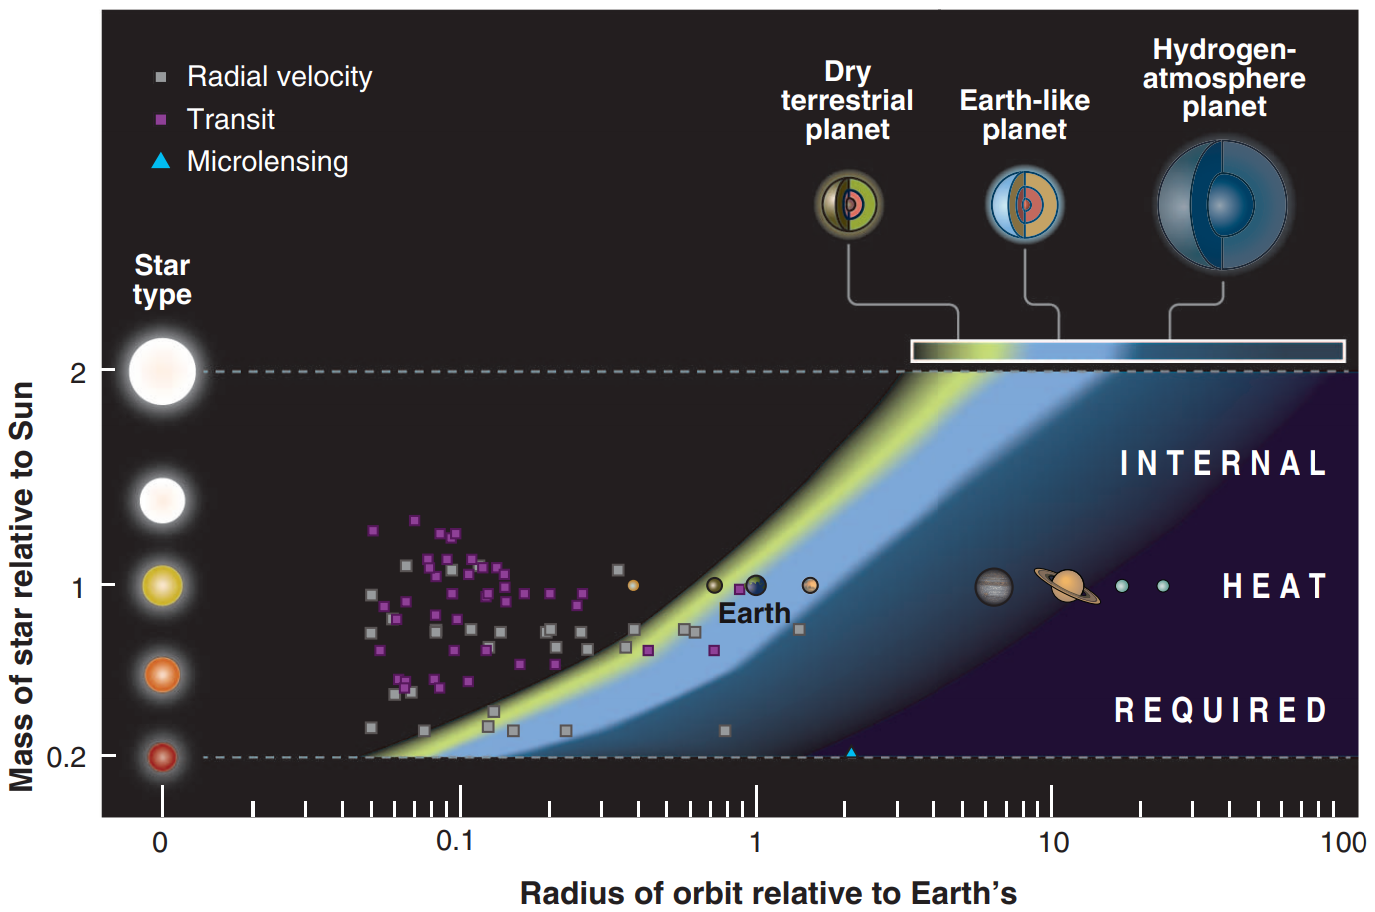
\includegraphics[width=1\textwidth]{Pic/Planets_habitability_Seager.png}
\caption{Seager representation of planet habitability as function of star type (that determinates the stellar activity) and planet distance. Image taken from \cite{seager2013exoplanet}}
\label{Planets_habitability_Seager}
\end{center}
\end{figure}






\section{R code}
\begin{lstlisting}


\end{lstlisting}
%------------------------------------------------



%----------------------------------------------------------------------------------------
%	BIBLIOGRAPHY
%----------------------------------------------------------------------------------------

\renewcommand{\refname}{\spacedlowsmallcaps{References}} % For modifying the bibliography heading

\bibliographystyle{unsrt}

\bibliography{bibliography.bib} % The file containing the bibliography

%----------------------------------------------------------------------------------------

\end{document}